%% Baseado no arquivo: 
%% abtex2-modelo-trabalho-academico.tex, v-1.9.6 laurocesar
%% by abnTeX2 group at http://www.abntex.net.br/ 
%% Adaptado para um modelo dssse TCC (Graduação)

% ------------------------------------------------------------------------
% ------------------------------------------------------------------------
% abnTeX2: Modelo de Trabalho Academico (tese de doutorado, dissertacao de
% mestrado e trabalhos monograficos em geral) em conformidade com 
% ABNT NBR 14724:2011: Informacao e documentacao - Trabalhos academicos -
% Apresentacao
% ------------------------------------------------------------------------
% ------------------------------------------------------------------------

\documentclass[
	% -- opções da classe memoir --
	12pt,				% tamanho da fonte,			% capítulos começam em pág ímpar (insere página vazia caso preciso)
	oneside,			% para impressão em recto e verso. Oposto a oneside
	a4paper,			% tamanho do papel. 
	% -- opções da classe abntex2 --
	%chapter=TITLE,		% títulos de capítulos convertidos em letras maiúsculas
	%section=TITLE,		% títulos de seções convertidos em letras maiúsculas
	%subsection=TITLE,	% títulos de subseções convertidos em letras maiúsculas
	%subsubsection=TITLE,% títulos de subsubseções convertidos em letras maiúsculas
	% -- opções do pacote babel --
	english,			% idioma adicional para hifenização
	%french,				% idioma adicional para hifenização
	%spanish,			% idioma adicional para hifenização
	brazil				% o último idioma é o principal do documento
	]{abntex2}

% ---
% Pacotes básicos 
% ---
\usepackage{pdflscape}
\usepackage{afterpage}
\usepackage{changepage}
\usepackage{capt-of}% or use the larger `caption` package
\usepackage{longtable}
\usepackage{dsfont}
\usepackage{float}
\usepackage{eucal}
\usepackage{lmodern}
\usepackage{amssymb}			% Usa a fonte Latin Modern			
\usepackage[T1]{fontenc}		% Selecao de codigos de fonte.
\usepackage[utf8]{inputenc}		% Codificacao do documento (conversão automática dos acentos)
\usepackage{lastpage}			% Usado pela Ficha catalográfica
\usepackage{indentfirst}		% Indenta o primeiro parágrafo de cada seção.
\usepackage{color}				% Controle das cores
\usepackage{graphicx}			% Inclusão de gráficos
\usepackage{microtype} 	% para melhorias de justificação
\usepackage{makecell}
\usepackage{tikz}
\usepackage{listings}
\usepackage{color}
\usepackage[nounderscore]{syntax}
\usepackage{etoolbox} % for patching
\usepackage{graphicx}


\definecolor{dkgreen}{rgb}{0,0.6,0}
\definecolor{gray}{rgb}{0.5,0.5,0.5}
\definecolor{mauve}{rgb}{0.58,0,0.82}

\lstset{
  literate=%
        {ã}{{\~{a}}}1
        {ç}{{\c{c}}}1,
  numbers=left,
  xleftmargin=2em,
  frame=single,
  framexleftmargin=1.5em,
  language=Java,
  aboveskip=3mm,
  belowskip=3mm,
  showstringspaces=false,
  columns=flexible,
  basicstyle={\small\ttfamily},
  numberstyle=\color{gray},
  keywordstyle=\color{blue},
  commentstyle=\color{dkgreen},
  stringstyle=\color{mauve},
  breaklines=true,
  breakatwhitespace=true,
  tabsize=3
}



\makeatletter
% define the main command on the model of the original one
% we add stepping the counter and typesetting the number
\def\gr@implnumbereditem<#1> #2 {%
  \stepcounter{grammarline}%
  \sbox\z@{\hskip\labelsep\grammarlabel{#1}{#2}}
  \strut\@@par%
  \vskip-\parskip%
  \vskip-\baselineskip%
  \hrule\@height\z@\@depth\z@\relax%
  \item[%
    \rlap{\hskip\dimexpr\linewidth+\grammarindent\relax %% add the number
          \llap{(\thegrammarline)}}%
    \unhbox\z@]%
  \catcode`\<\active%
}
% copy the grammar environment under a new name
\let\numberedgrammar\grammar
\let\endnumberedgrammar\endgrammar
% now patch the new environment
\pretocmd\numberedgrammar{\setcounter{grammarline}{0}}{}{}
\patchcmd\numberedgrammar
  {\gr@implitem}
  {\gr@implnumbereditem}
  {}{}
\patchcmd\numberedgrammar
  {\def\alt{\\\llap{\textbar\quad}}}
  {\let\alt\alt@num}
  {}{}

% the command for numbering the \alt lines
\def\alt@num{\\\relax
  \stepcounter{grammarline}%
  \rlap{\hskip\dimexpr\linewidth-\labelwidth+\grammarindent-\labelsep\relax
        \llap{(\thegrammarline)}}% add the number
  \llap{\textbar\quad}}

\newcounter{grammarline}
\makeatother
% ---
		

% ---
% Pacotes de citações
% ---
\usepackage[brazilian,hyperpageref]{backref}	 % Paginas com as citações na bibl
\usepackage[alf]{abntex2cite}	% Citações padrão ABNT

% --- 
% CONFIGURAÇÕES DE PACOTES
% --- 

% ---
% Configurações do pacote backref
% Usado sem a opção hyperpageref de backref
\renewcommand{\backrefpagesname}{%Citado na(s) página(s):~
}
% Texto padrão antes do número das páginas
\renewcommand{\backref}{}
% Define os textos da citação
\renewcommand*{\backrefalt}[4]{
	%\ifcase #1 %
	%	Nenhuma citação no texto.%
	%\or
	%	Citado na página #2.%
	%\else
	%	Citado #1 vezes nas páginas #2.%
	%\fi
    }%
% ---

% ---
% Informações de dados para CAPA e FOLHA DE ROSTO
% ---
\titulo{KPiler: compilador para a linguagem K}
\autor{Josué Rocha Lima}
\local{Belo Horizonte}
\data{2017}
\orientador{Kecia Aline Marques Ferreira}

\instituicao{%
  Centro Federal de Educação Tecnológica de Minas Gerais
  \par
  Departamento de Computação
  \par
  Curso de Engenharia de Computação
  }
\tipotrabalho{Monografia (Graduação)}
% O preambulo deve conter o tipo do trabalho, o objetivo, 
% o nome da instituição e a área de concentração 
\preambulo{Relatório do trabalho prático apresentado à disciplina de compiladores.}
% ---


% ---
% Configurações de aparência do PDF final

% alterando o aspecto da cor azul
\definecolor{blue}{RGB}{41,5,195}

% informações do PDF
\makeatletter
\hypersetup{
     	%pagebackref=true,
		pdftitle={\@title}, 
		pdfauthor={\@author},
    	pdfsubject={\imprimirpreambulo},
	    pdfcreator={LaTeX with abnTeX2},
		pdfkeywords={abnt}{latex}{abntex}{abntex2}{trabalho acadêmico}, 
		colorlinks=true,       		% false: boxed links; true: colored links
    	linkcolor=blue,          	% color of internal links
    	citecolor=blue,        		% color of links to bibliography
    	filecolor=magenta,      		% color of file links
		urlcolor=blue,
		bookmarksdepth=4
}
\makeatother
% --- 

% --- 
% Espaçamentos entre linhas e parágrafos 
% --- 

% O tamanho do parágrafo é dado por:
\setlength{\parindent}{1.3cm}

% Controle do espaçamento entre um parágrafo e outro:
\setlength{\parskip}{0.2cm}  % tente também \onelineskip

% ---
% compila o indice
% ---
\makeindex
% ---

% ----
% Início do documento
% ----
\begin{document}

% Seleciona o idioma do documento (conforme pacotes do babel)
%\selectlanguage{english}
%\selectlanguage{brazil}

% Retira espaço extra obsoleto entre as frases.
\frenchspacing 

% ----------------------------------------------------------
% ELEMENTOS PRÉ-TEXTUAIS
% ----------------------------------------------------------



%% Baseado no arquivo: 
%% abtex2-modelo-trabalho-academico.tex, v-1.9.6 laurocesar
%% by abnTeX2 group at http://www.abntex.net.br/ 
%% Adaptado para um modelo de TCC (Graduação)

% ---
% Capa
% ---
%\imprimircapa
% ---

% ---
% Folha de rosto
% (o * indica que haverá a ficha bibliográfica)
% ---
\imprimirfolhaderosto*
% ---

% ---
% Inserir a ficha bibliografica
% ---

% Isto é um exemplo de Ficha Catalográfica, ou ``Dados internacionais de
% catalogação-na-publicação''. Você pode utilizar este modelo como referência. 
% Porém, provavelmente a biblioteca da sua universidade lhe fornecerá um PDF
% com a ficha catalográfica definitiva após a defesa do trabalho. Quando estiver
% com o documento, salve-o como PDF no diretório do seu projeto e substitua todo
% o conteúdo de implementação deste arquivo pelo comando abaixo:
%
% \begin{fichacatalografica}
%     
% \end{fichacatalografica}

\begin{fichacatalografica}
~
%\includepdf{fig_ficha_catalografica.pdf}
% 	\sffamily
% 	\vspace*{\fill}					% Posição vertical
% 	\begin{center}					% Minipage Centralizado
% 	\fbox{\begin{minipage}[c][8cm]{13.5cm}		% Largura
% 	\small
% 	\imprimirautor
% 	%Sobrenome, Nome do autor
	
% 	\hspace{0.5cm} \imprimirtitulo  / \imprimirautor. --
% 	\imprimirlocal, \imprimirdata-
	
% 	\hspace{0.5cm} \pageref{LastPage} p. : il. (algumas color.) ; 30 cm.\\
	
% 	\hspace{0.5cm} \imprimirorientadorRotulo~\imprimirorientador\\
	
% 	\hspace{0.5cm}
% 	\parbox[t]{\textwidth}{\imprimirtipotrabalho~--~\imprimirinstituicao,
% 	\imprimirdata.}\\
	
% 	\hspace{0.5cm}
% 		1. Palavra-chave1.
% 		2. Palavra-chave2.
% 		2. Palavra-chave3.
% 		I. Orientador.
% 		II. Universidade xxx.
% 		III. Faculdade de xxx.
% 		IV. Título 			
% 	\end{minipage}}
% 	\end{center}
\end{fichacatalografica}
% ---

% % ---
% % Inserir errata
% % ---
% \begin{errata}
% Elemento opcional da \citeonline[4.2.1.2]{NBR14724:2011}. Exemplo:

% \vspace{\onelineskip}

% FERRIGNO, C. R. A. \textbf{Tratamento de neoplasias ósseas apendiculares com
% reimplantação de enxerto ósseo autólogo autoclavado associado ao plasma
% rico em plaquetas}: estudo crítico na cirurgia de preservação de membro em
% cães. 2011. 128 f. Tese (Livre-Docência) - Faculdade de Medicina Veterinária e
% Zootecnia, Universidade de São Paulo, São Paulo, 2011.

% \begin{table}[htb]
% \center
% \footnotesize
% \begin{tabular}{|p{1.4cm}|p{1cm}|p{3cm}|p{3cm}|}
%   \hline
%    \textbf{Folha} & \textbf{Linha}  & \textbf{Onde se lê}  & \textbf{Leia-se}  \\
%     \hline
%     1 & 10 & auto-conclavo & autoconclavo\\
%    \hline
% \end{tabular}
% \end{table}

% \end{errata}
% ---

% ---
% Inserir folha de aprovação
% ---


%
%\begin{folhadeaprovacao}

%  \begin{center}
%    Espaço destinado à folha de aprovação
%após aprovação, insira a cópia da folha de aprovação por meio do comando:
% \includepdf{folhadeaprovacao_final.pdf}
%  \end{center}
  
%\end{folhadeaprovacao}
% ---

% ---
% Dedicatória
% ---
%\begin{dedicatoria}
%   \vspace*{\fill}
%   \centering
%   \noindent
%   \textit{Dedico este trabalho aos alunos(as) do CEFET-MG.} \vspace*{\fill}
%\end{dedicatoria}
% ---

% ---
% Agradecimentos
% ---
%\begin{agradecimentos}
%Agradeço ao Latex e às pessoas que contribuiram com o desenvolvimento do Abntex2 por facilitarem a vida dos graduandos.
%\end{agradecimentos}
% ---

% ---
% Epígrafe
% ---
%\begin{epigrafe}
%    \vspace*{\fill}
%	\begin{flushright}
%		\textit{``As pessoas costumam dizer que a motivação não dura sempre. Bem, nem o efeito do banho, por isso recomenda-se diariamente.''\\
%		(Zig Ziglar)}
%	\end{flushright}
%\end{epigrafe}
% ---

% ---
% RESUMOS
% ---



% resumo em inglês
%\begin{resumo}[Abstract]
% \begin{otherlanguage*}{english}
%   This is the abstract of your undergraduate thesis. 
%   Here is important to contextualize and present your problem, motivation and the goal of your work. After that, you need to present the results, contributions and conclusions of your study.

%   \vspace{\onelineskip}
 
%   \noindent 
%   \textbf{Keywords}: latex. abntex. text editoration.
% \end{otherlanguage*}
%\end{resumo}


% ---

% ---
% inserir lista de ilustrações
% ---
%\pdfbookmark[0]{\listfigurename}{lof}
%\listoffigures*
%\cleardoublepage
% ---

% ---
% inserir lista de tabelas
% ---
%\pdfbookmark[0]{\listtablename}{lot}
%\listoftables*
%\cleardoublepage
% ---

% ---
% inserir lista de abreviaturas e siglas
% ---
%\begin{siglas}
%  \item[ABNT] Associação Brasileira de Normas Técnicas
%  \item[abnTeX] ABsurdas Normas para TeX
%\end{siglas}
% ---

% ---
% inserir lista de símbolos
% ---
%\begin{simbolos}
%  \item[$ \Gamma $] Letra grega Gama
%  \item[$ \Lambda $] Lambda
%  \item[$ \zeta $] Letra grega minúscula zeta
%  \item[$ \in $] Pertence
%\end{simbolos}
% ---

% ---
% inserir o sumario
% ---
\pdfbookmark[0]{\contentsname}{toc}


\tableofcontents*

\cleardoublepage
% ---

% ----------------------------------------------------------
% ELEMENTOS TEXTUAIS
% ----------------------------------------------------------
\textual

% ----------------------------------------------------------
% Como o documento será grande, sugiro dividir em diversos arquivos, um para cada capítulo.
% ----------------------------------------------------------



\chapter[Introdução]{Introdução}
\label{cap:introducao}



Com o intuito de reduzir a complexidade da implementação de sistemas de software, foi proposta a utilização de linguagens próximas da linguagem humana, denominadas linguagens de alto nível. Entretanto, para possibilitar a implementação de software dessa maneira, é necessário a tradução para uma linguagem que possa ser executada diretamente no \textit{hardware} \cite{aho2007compilers}.

O compilador é um sistema de \textit{software} responsável pela tradução automática de um programa em linguagem fonte de alto nível, para um programa semanticamente equivalente em uma linguagem alvo, conforme pode-se observar na Figura \ref{fig:compiler}. Deste modo, os compiladores são considerados \textit{software} básico para a computação.

\begin{figure}[!h]
\label{fig:compiler}
\centering
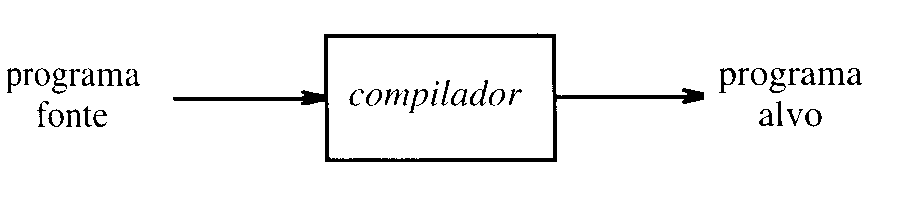
\includegraphics[width=12cm,height=12cm,keepaspectratio]{img/compiler.png}
\caption{Tradução do programa fonte para a linguagem alvo realizada pelo compilador \cite{aho2007compilers}.}
\end{figure}

O compilador é comumente dividido em módulos para reduzir a complexidade do seu processo de implementação. Essa divisão é frequentemente compreendida pelos seguintes módulos:

\begin{itemize}
    \item \textbf{Front-end (Análise)}
    \begin{itemize}
        \item \textbf{Analisador léxico}: lê o programa fonte caractere a caractere e agrupa o programa em sequências significativas denominadas lexemas. Para cada um dos lexemas é gerado um \textit{token} no formato <nome , valor>. O analisador léxico também é responsável por reconhecer e ignorar comentários e gerenciar numeração de linhas.
        \item \textbf{Analisador sintático}: recebe o fluxo de \textit{tokens} gerado pelo analisador sintático e verifica se a sequência está de acordo com a estrutura sintática da linguagem. É o núcleo do compilador.
        \item \textbf{Analisador semântico}: Utiliza a tabela de símbolos e árvore sintática para verificar se o programa-fonte atende às regras semânticas da linguagem, como regras de compatibilidade de tipos.
        \item \textbf{Gerador de código intermediário:} Código em representação intermediária em baixo nível é gerado para auxiliar a geração de código e otimização.
    \end{itemize}
    \item \textbf{Back-end (Síntese)}
    \begin{itemize}
        \item \textbf{Gerador de código:} mapeia a linguagem intermediária para a linguagem objeto. 
    \end{itemize}
\end{itemize}

A Figura \ref{fig:flow_modules} ilustra o fluxo entre os módulos do compilador:

\begin{figure}[!h]
\label{fig:flow_modules}
\centering
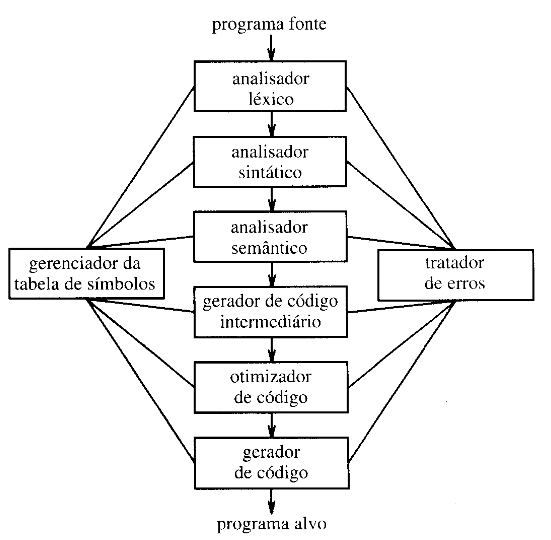
\includegraphics[width=10cm,height=10cm,keepaspectratio]{img/flow.png}
\caption{Divisão em módulos do compilador \cite{aho2007compilers}.}
\end{figure}


\section{Proposta de trabalho prático}

Foi proposto o projeto e implementação de um compilador para uma linguagem hipotética \textit{K} como trabalho prático e didático para a disciplina de Compiladores. Devido à complexidade do problema de compilação, o projeto foi dividido em quatro componentes com suas respectivas entregas:

\begin{enumerate}
    \item \label{lexico} Analisador léxico e tabela de símbolos;
    \item Analisador sintático;
    \item Analisador semântico;
    \item Gerador de código.
    
\end{enumerate}

O trabalho entregue anexo à este relatório corresponde ao analisador sintático (2). Linguagens de programação possuem regras precisas que descrevem sentenças aceitas na construção de um programa bem formado \cite{aho2007compilers}. O analisador sintático verifica se o programa-fonte submetido ao compilador está sintaticamente correto, isto é, se as ordens dos \textit{tokens} casam com as regras especificadas para a linguagem.

A organização e disposição sintática dos elementos de uma linguagem de programação é especificada por gramáticas livres de contexto. Como especificação para a linguagem \textit{K}, foi fornecida uma gramática no formato Formalismo de Backus-Naur Extendido (EBNF, do inglês \textit{Extended Backus-Naur Form}).

Deste modo, o analisador sintático recebe o fluxo de \textit{tokens} gerado pelo analisador léxico e verifica se sua ordem casa com as regras especificadas na gramática. Foi solicitado a implementação do reconhecimento das regras sintáticas especificados na gramática e identificação de erros sintáticos.

Foi proposta implementação de um analisador sintático descendente, cujo nome se origina do processo de derivação da entrada. A arvore sintática é construída de cima para baixo, produzindo uma derivação mais à esquerda para a cadeia de entrada.

O \textit{parser} recursivo descendente utiliza uma série de procedimentos recursivos, que são gerados para cada símbolo não terminal da gramática que contêm pontos de decisão de acordo com cada elemento que o respectivo símbolo não-terminal possa produzir.  

Entretanto, para que seja possível implementar este \textit{parser}, é necessário que a gramática que especifica as regras da linguagem seja classificada como LL(1). O nome indíca que a cadeia é lida da esquerda para a direita (primeiro L), é realizada um derivação mais à esquerda (segundo L) e só é necessário conhecer um único símbolo a frente para a tomada de decisões.

Para que seja classificada como LL(1), é necessário que dada gramática não contenha recursão à esquerda e produções com prefixo comum. Pode-se verificar se é possível implementar um \textit{parser} recursivo descendente para dada gramática por meio da geração de um projeto que tem como produto final a tabela do \textit{parser}. Caso não existam entradas múltiplas na tabela do \textit{parser}, a gramática é denominada LL(1). A geração da tabela do parser é realizada baseado nos conjuntos \textit{first} e \textit{follow} de cada não-terminal.

A metodologia e principais decisões tomadas nesse trabalho se encontra detalhada no Capítulo \ref{cap:metodologia}.



\chapter[Metodologia]{Metodologia}
\label{cap:metodologia}

Para verificação da conformidade do programa-fonte com as regras sintáticas da linguagem \textit{K}, foi desenvolvido um analisador sintático descendente. Foi construído um projeto para o \textit{parser} com o intuito de facilitar o desenvolvimento e  evitar descoberta de peculiaridades da implementação em uma fase tardia da mesma.

\section{Projeto do analisador sintático}
\label{sec:metodologia_projeto}

Inicialmente, foi realizado um estudo da gramática da linguagem \textit{K}, com o intuito de identificar produções que não possuem características LL(1), isto é, recursão à esquerda e prefixos comuns. Após identificação destas características, as produções que continham as mesmas foram adaptadas para atender aos requisitos de uma gramática LL(1). As alterações realizadas consistiram nos seguintes aspectos:

\begin{itemize}
    \item Adição de um ponto de partida contendo o símbolo inicial original seguido de \$ (fim de arquivo);
    \item Decomposição de regras com recursão à esquerda em duas regras para transformar em recursão à direita;
    \item Adiamento da tomada de decisão em produções com prefixo comum por meio da criação de uma regra específica para o ponto de decisão.
\end{itemize}

A gramática obtida após as adaptações pode ser observada a seguir:

\begin{numberedgrammar}

<program\_prime> ::= <Program> `\$' 

<Program> ::= 'program' <decllist> <stmt-list> 'end' 

<decllist> ::= <decl-list> 
\alt `\lambda' 
    
<decl-list> ::= <decl> <decllist>

<decl> ::= <type> <identifier-list> ;

<identifier-list> ::= <identifier> <possible-ident>

<possible-ident> ::= `,' <identifier> <possible-ident> 
\alt `\lambda' 

<type> ::= <int> 
\alt <string>

<stmt-list> ::= <stmt> <stmtlist>

<stmtlist> ::= <stmt-list> 
\alt `\lambda'

<stmt> ::=   <assign-stmt> ; 
\alt <if-stmt> 
\alt <while-stmt> 
\alt <read-stmt> ';' 
\alt <write-stmt> ';'
	
<assign-stmt> ::= <identifier> '=' <simple-expr>

<if-stmt> ::= 'if' <condition> 'then' <stmt-list> <if-stmt-prime>

<if-stmt-prime> ::=   'end' 
\alt 'else' <stmt-list> <end>
		 
<condition> ::= <expression>

<while-stmt> ::= 'do' <stmt-list> <stmt-sufix>

<stmt-sufix> ::= 'while' <condition> 'end'

<read-stmt> ::= 'scan' '(' <identifier> ')'

<write-stmt> ::= <print> '(' <writable> ')'

<writable> ::= <simple-expr> 
\alt <literal>

<expression> ::= <simple-expr> <expression-prime>

<expression-prime> ::= <relop> <simple-expr> 
\alt `\lambda'

<simple-expr> ::= <term> <simple-expr-prime>

<simple-expr-prime> ::= 	  <addop> <term> <simple-expr-prime> 
\alt `\lambda'

<term> ::= <factor-a> <term-prime>

<term-prime> ::=   <mulop> <factor-a> <term-prime> 
\alt `\lambda'

<factor-a> ::= <factor> 
\alt '!' <factor> 
\alt '-' <factor>

<factor> ::= <identifier> 
\alt <constant> 
\alt '(' <expression> ')'

<relop> ::= '==' 
\alt `>' 
\alt `>=' 
\alt `<' 
\alt `<=' 
\alt `!='

<addop> ::= `+' 
\alt `-' 
\alt `||'

<mulop> ::= `*' 
\alt `/' 
\alt `&&'

\end{numberedgrammar}


Para possibilitar a implementação da metodologia proposta, os \textit{tokens} especificados na gramática da linguagem \textit{K} foram identificados e seus conjuntos \textit{FIRST} e \textit{FOLLOW} foram calculados (Tabela \ref{table:tokens}):

\begin{longtable}{|c | c | c|} 

\hline
 \textbf{Token} & \textbf{Conjunto \textit{FIRST}} & \textbf{Conjunto \textit{FOLLOW}} \\ 
 \hline
 Program & \makecell{program} &  \makecell{\$}\\ 
 \hline
 decllist & \makecell{\lambda, int, string} & \makecell{identifier, do, print, if, scan} \\ 
 \hline
 decl-list & int, string & identifier, do, print, if, scan \\ 
 \hline
 decl & int, string & \makecell{int, string, identifier, do, print, if, scan} \\ 
 \hline
 identifier-list & identifier & ;\\
 \hline
 possible-ident  & ",", \lambda & 	;\\
 \hline
 type  & int, string & identifier \\
 \hline
 stmtlist  & \makecell{\lambda, identifier,\\ do, print, if, scan} & while, end, else\\
 \hline
 assign-stmt & identifier & ;\\
 \hline
 if-stmt & if & \makecell{identifier, do, print, if,\\ scan, while, end, else}\\
 \hline
 if-stmt-prime & end, else & \makecell{identifier, do, print, if,\\ scan, while, end, else}\\
 \hline
 while-stmt & do & \makecell{identifier, do, print, if,\\ scan, while, end, else}\\
 \hline
 stmt-sufix & while & \makecell{identifier, do, print, if,\\ scan, while, end, else}\\
  \hline
 read-stmt & scan & ;\\
  \hline
 write-stmt & print & ;\\
\hline
 writable &	\makecell{literal, !, -, identifier,\\ (, integer-const} & )\\
 \hline
 simple-expr-prime & \lambda, +, -, ||  & \makecell{==, >, >=, <, <=, !=,\\ ), end, then, ;}\\
 \hline
 term-prime &	\lambda, *, /, \&\&  &  \makecell{+, -, ||, ==, >, >=,\\ <, <=, !=, ), end, then, ;}\\
 \hline
 factor-a &	\makecell{!, -, identifier, (,\\ \detokenize{integer_const}, literal} & \makecell{*, /, \&\&, +, -, ||,\\ ==, >, >=, <,\\ <=, !=, ), end, then, ;} \\
 \hline
 factor	& \makecell{identifier, (, \detokenize{integer_const},\\ literal} & \makecell{*, /, \&\&, +, -,\\ ||, ==, >, >=, <,\\ <=, !=, ), end, then, ;} \\
 \hline
 relop	& \makecell{==, >, >=, <,\\ <=, !=} & \makecell{!, -, identifier, (,\\ \detokenize{integer_const}, literal} \\
 \hline
 addop	& \makecell{+, -, ||} & \makecell{!, -, identifier, (,\\ \detokenize{integer_const}, literal} \\
 \hline
 mulop	& \makecell{*, /, \&\&} & \makecell{!, -, identifier, (,\\ \detokenize{integer_const}, literal} \\
 \hline
 constant &	\makecell{\detokenize{integer_const}, literal} & \makecell{*, /, \&\&, +, -,\\ ||, ==, >, >=, <,\\ <=, !=, ), end,\\ then, ;}\\
 \hline
 stmt & \makecell{identifier, do, print,\\ if, scan} & \makecell{identifier, do, print, if,\\ scan, while, end, else}\\
 \hline 
 term &	\makecell{!, -, identifier,\\ (, \detokenize{integer_const}, literal} & \makecell{+, -, ||, ==,\\ >, >=, <, <=, !=,\\ ), end, then, ;}\\
 \hline
 stmt-list	& \makecell{identifier, do, print,\\ if, scan} & while, end, else \\
 \hline
 simple-expr & \makecell{!, -, identifier, (,\\ \detokenize{integer_const}, literal} & \makecell{==, >, >=, <, <=,\\ !=, ), end, then, ;} \\
 \hline
 expression &	\makecell{!, -, identifier, (,\\ integer-const, literal} & \makecell{), end, then}\\
 \hline
 expression-prime &	\makecell{\lambda, ==, >, >=, <, <=, !=} & \makecell{), end, then}\\
 \hline
 
 condition & \makecell{!, -, identifier, (,\\ integer\_const, literal} & \makecell{end, then}\\
 \hline
 
\caption{Produções e seus conjuntos \textit{first} e \textit{follow}.}
\label{table:tokens}
\end{longtable}

Após o cálculo dos conjuntos \textit{first} e follow dos símbolos não-terminais, os mesmos (juntamente com a gramática modificada) foram utilizados para construir a tabela do \textit{parser}. É possível observar que a tabela não possui entradas duplicadas. Portanto, é possível implementar um \textit{parser} recursivo descendente para a mesma. A tabela do \textit{parser} foi movida para a próxima página para facilitar sua visualização.

\afterpage{
    \clearpage
    \thispagestyle{empty}% empty page style (?)
    \begin{landscape}% Landscape page
    \fontsize{10}{10}\selectfont
    \begin{adjustwidth}{-2cm}{}

        \centering % Center table
        \begin{tabular}{|c | c | c| c | c | c | c | c | c |c | c | c| c | c | c | c | c | c | c |}
          \hline
 \textbf{Produção} & \textbf{\$} & \textbf{program} & \textbf{end} & \textbf{identifier} & \textbf{,} & \textbf{int} & \textbf{string} & \textbf{;} & \textbf{=} & \textbf{if} & \textbf{then} & \textbf{else} & \textbf{do} & \textbf{while} & \textbf{scan} & \textbf{(} & \textbf{)} & \textbf{print} \\ 
 \hline
 Program & & 2 & & & &  & & & & & & & & & & & &\\ 
 \hline
 decllist & & & & 3 &  &  & & &  & 4 & &  & 4 &  & 4 & & & 4\\ 
 \hline
 decl-list & & & & 5 &  &  & & &  &  & &  &  &  &  & & & \\ 
 \hline
  decl & & & & 6 &  &  & & &  &  & &  &  &  &  & & & \\ 
   \hline
  identifier-list & & & & 7 &  &  & & &  &  & &  &  &  &  & & & \\ 
 \hline
possible-ident & & & &  & 8 &  & & &  & 8 &  &  & 8 & & 8 & & & 9 \\ 
 \hline
 type & & & &  &  & 10 & 11 & &  &  &  &  &  & & 8 & & &  \\ 
 \hline
  stmtlist & & & 14 & 13 &  &  &  & &  & 13 &  & 14 & 12 & 14 & 13 & & & 13  \\ 
 \hline
   stmt-list & & &  & 12 &  &  &  & &  & 12 &  &  & 12 &  & 12 & & & 12  \\ 
 \hline
 
  stmt & & &  & 15 &  &  &  & &  & 16 &  &  & 17 &  & 18 & & & 19  \\ 
 \hline
  assign-stmt & & &  & 20 &  &  &  & &  &  &  &  &  &  &  & & &   \\ 
 \hline
  assign-stmt & & &  & 20 &  &  &  & &  &  &  &  &  &  &  & & &   \\ 
 \hline
  if-stmt & & &  &  &  &  &  & &  & 21 &  &  &  &  &  & & &   \\ 
 \hline 
  if-stmt-prime & & & 22 &  &  &  &  & &  &  &  & 23 &  &  &  & & &   \\ 
 \hline
  condition & & & & 24 & & & & & & & & & & & & 24 & &   \\ 
 \hline
 while-stmt & & & & & & & & & & & & & 25 & & & & &   \\ 
 \hline
 stmt-sufix & & & & & & & & & & & & & & 26 & & & &   \\ 
\hline
 read-stmt & & & & & & & & & & & & & & & 27 & & &   \\ 
\hline
 write-stmt & & & & & & & & & & & & & & & & & & 28  \\ 
\hline
 write-stmt & & & & & & & & & & & & & & & & & & 28  \\ 
\hline
 writable & & & & 29 & & & & & & & & & & & & 29 & &  \\
 \hline
 expression & & & & 31 & & & & & & & & & & & & 31 & &  \\
 \hline
 expression-prime & & & 33 & & & & & & & & 32 & & & & & & 32 & \\
 \hline
 simple-expr & & & & 34 & & & & & & & & & & & & 34 & & \\
 \hline
 simple-expr-prime & & & 36 &  & & & & & & & 36 & & & & & 34 & 36 & \\
 \hline
 term & & &  & 37 & & & & & & &  & & & & & 37 &  & \\
 \hline
 term-prime & & & 39 & & & & & & & & 39 & & & & & & 39 & \\
 \hline
 factor-a & & & & 40 & & & & & & & & & & & & 40 & & \\
 \hline
 factor & & & & 43 & & & & & & & & & & & & 45 & & \\
 
 \hline\\
        \end{tabular}
        \captionof{table}{Primeira parte da tabela do parser LL(1)}% Add 'table' caption
    \end{adjustwidth}{}{}
    \end{landscape}
    \clearpage% Flush page
}




\afterpage{
    \clearpage
    \thispagestyle{empty}% empty page style (?)
    \begin{landscape}% Landscape page
    \fontsize{10}{10}\selectfont
    \begin{adjustwidth}{-2cm}{}
        \centering % Center table

        \begin{tabular}{|c | c | c| c | c | c | c | c | c |c | c | c| c | c | c | c |}
          \hline
 \textbf{literal} & \textbf{!} & \textbf{-} & \textbf{==} & \textbf{>} & \textbf{>=} & \textbf{<} & \textbf{<=} & \textbf{!=} & \textbf{+} & \textbf{||} & \textbf{*} & \textbf{/} & \makecell{\textbf{\&\&}} & \textbf{integer-const} & \textbf{literal} \\ 
 \hline
  condition & 24 & 24 & & & & & & & & & & & & 24 & 24\\ 
 \hline
 while-stmt & & & & & & & & & & & & & & & \\
 \hline
 stmt-sufix & & & & & & & & & & & & & & &    \\ 
\hline
 read-stmt & & & & & & & & & & & & & & &   \\ 
\hline
 write-stmt & & & & & & & & & & & & & & &  \\ 
\hline
 write-stmt & & & & & & & & & & & & & & &   \\ 
\hline
 writable & 29 & 29 & & & & & & & & & & & & 29 & 30  \\
\hline
 expression & 31 & 31 & & & & & & & & & & & & 31 & 31  \\
 \hline
 expression-prime & & & 32 & 32 & 32 & 32 & 32 & 32 & & & & & & &  \\
 \hline
simple-expr & 34 & 34 & & & & & & & & & & & & 34 & 34  \\
\hline
simple-expr-prime & & 35 & 36 & 36 & 36 & 36 & 36 & 36 & 35 & 35 & & & & &   \\
 \hline
term & 37 & 37 &  &  &  & & & & & & & & & 37 & 37  \\
 \hline
term &  & 39 & 39 & 39 & 39 & 39 & 39 & 39 & 39 & 39 & 38 & 38 & 38 &  &   \\
\hline
factor-a & 41 & 42 & & & & & & & & & & & & 40 & 40  \\
\hline
factor &  &  & & & & & & & & & & & & 44 & 44  \\
\hline
relop & & & 46 & 47 & 48 & 49 & 50 & 51 & & & & & & 44 & 44  \\
\hline
addop & & 53 & & & & & & & 52 & 54 & & & & &   \\
\hline
mulop & & & & & & & & & & & 55 & 56 & 57 & & \\
\hline


 \hline  \\
        \end{tabular}
        \captionof{table}{Segunda parte da tabela do parser LL(1)}% Add 'table' caption
    \end{adjustwidth}{}{}
    \end{landscape}
    \clearpage% Flush page
}




\newpage
\section{Implementação do analisador sintático}

A linguagem de programação Java foi escolhida para a implementação do analisador sintático do compilador em continuação a implementação prévia do primeiro trabalho prático e devido aos recursos de processamento de texto e estruturas de dados disponíveis na linguagem, além de sua compilação híbrida que permite execução multiplataforma.

\subsection{Arquitetura da implementação}

  O diagrama de classe gerado no trabalho anterior(Figura \ref{fig:diagram}) foi atualizado para compreender as alterações e avanços realizados no projeto. A arquitetura do KPiler baseou-se nas diretrizes e recomendações de \cite{andrew2002modern}.

\begin{figure}[!h]
\centering
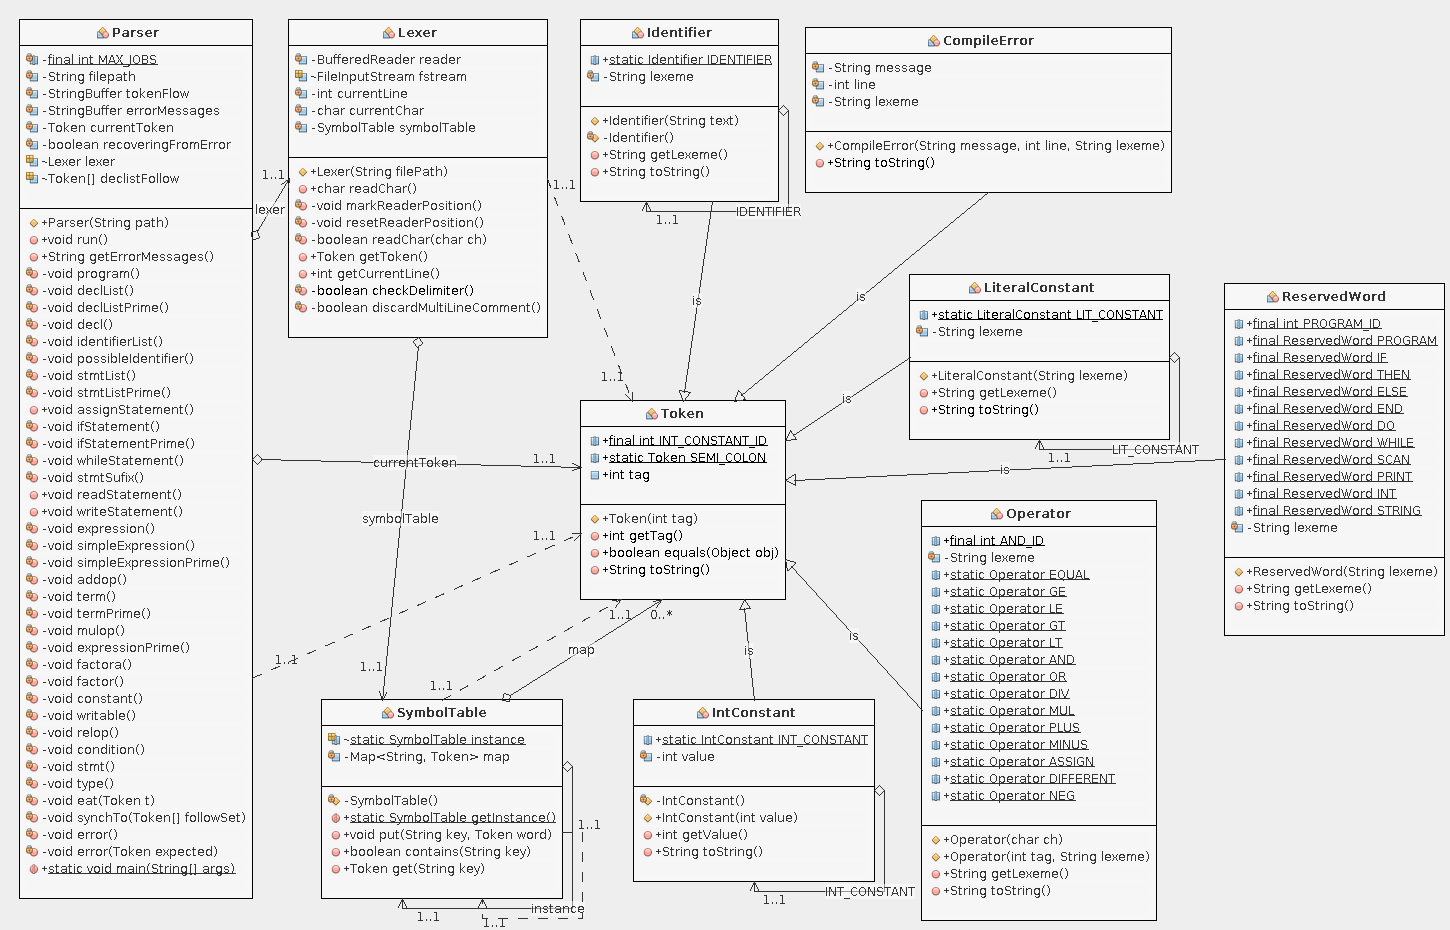
\includegraphics[width=16cm,height=20cm,keepaspectratio]{img/class_diagram.png}
\caption{Diagrama de classe do compilador, as classes utilitárias foram omitidas para facilitar o entendimento.}
\label{fig:diagram}
\end{figure}

Nesta etapa do projeto, somente as classes \textit{Token}, \textit{Lexer} e \textit{Parser} foram alteradas significativamente. Estas classes e funções estão detalhados a seguir:

\begin{itemize}
    \item \textbf{Parser (analisador sintático):} classe que contem o ponto de entrada (método \textit{main}) do programa. Uma requisição é feita à classe Lexer para obter o fluxo de \textit{tokens}, de modo à implementar compilação em um passo. A classe possui implementação multi-thread possibilitando processamento de vários arquivos simultaneamente. Para cada símbolo não-terminal da gramática foi implementado um método contendo as respectivas cláusulas da gramática. Os métodos \textit{error()}, \textit{synchTo(Token[] followSet)} e a \textbf{flag} booleana \textbf{recoveringFromError} foram utilizadas na implementação de erro em modo pânico.
    
    \item \textbf{Lexer (analisador léxico):} lê o programa fonte caractere a caractere, buscando sequências de caracteres significativas (lexemas) que casem com o padrão de algum \textit{token}. Possui estruturas para leitura do arquivo, armazenamento da linha corrente e um ponteiro para a tabela de símbolos. O método \textit{getToken()} contem a implementação dos autômatos para reconhecimento de \textit{tokens}. Nesta etapa do projeto, a mesma foi alterada para detectar símbolos não aceitos pela linguagem. Essa decisão foi movida pelo intuito de simplificar a implementação do analisador sintático delegando a responsabilidade de reconhecimento de símbolos não aceitos ao analisador léxico.
    
    \item \textbf{Token:} contem o dicionário de \textit{tags} e um atributo inteiro para armazenamento do mesmo. É classe pai das classes \textit{CompileError}, \textit{Identifier},\textit{IntConstant}, \textit{LiteralConstant}, \textit{ReservedWord} e \textit{Operator}. Estas classes implementam polimorfismo no método \textit{toString()} para exibir os \textit{tokens} em seu formato apropriado. Foi incorporado o método \textit{equal(Token t)} à classe \textit{Token} nesta etapa do trabalho para facilitar as comparações de igualdade.
    
\end{itemize}

\subsection{Recuperação de erro}

Com o intuito de exibir a maior quantidade de erros possível ao usuário, recuperação de erro em modo pânico foi implementada. Após ocorrência de um erro, \textit{tokens} são consumidos até que se encontre um \textit{token} de um conjunto especificado. Utilizou-se o conjunto \textit{follow} de cada não-terminal como heurística para recuperação de erro.

Com este recurso, foi possível exibir maior quantidade de erros em uma única compilação ao usuário. Os resultados da implementação podem ser observados no Capítulo \ref{cap:avaliacao} (Avaliação dos resultados).

\subsection{Recursos adicionais}

O compilador foi construído em uma arquitetura paralela, que permite que vários arquivos sejam analisados paralelamente pelos analisadores léxico e sintático. Para cada arquivo, são criados um objeto da classe \textit{Lexer} e um objeto da classe \textit{Parser} preservando a estrutura de compilação em um passo solicitada pela orientadora.

\chapter[Instruções de utilização]{Instruções de utilização}
\label{cap:instrucoes}

O projeto está preparado para receber o caminho dos arquivos de código-fonte via linha de comando (terminal do Linux ou \textit{prompt} de comandos do Windows). A passagem dos argumentos pode ser configurada no ambiente de desenvolvimento de preferência ou informado na inicialização do arquivo executável .jar ou na execução direta dos arquivos .class. Exemplo de execução:

\begin{itemize}
    \item \textbf{Execução do .jar:} o seguinte comando deve ser executado na mesma pasta do arquivo .jar caso as configurações do projeto anexado sejam mantidas:
    
    \begin{center}
        \textbf{java -jar KPiler.jar test/test1.k test/test1.k}
    \end{center}

    \item \textbf{Execução dos arquivos .class:} deve-se navegar para a pasta do \textit{build} e executar os seguintes comandos para compilar e executar o código:
    
    \begin{center}
        \textbf{javac Parser.java}
        
        \textbf{java Parser test/test1.k test/test1.k}
    \end{center}

\end{itemize}


\begin{figure}[!h]
\label{fig:execution}
\centering
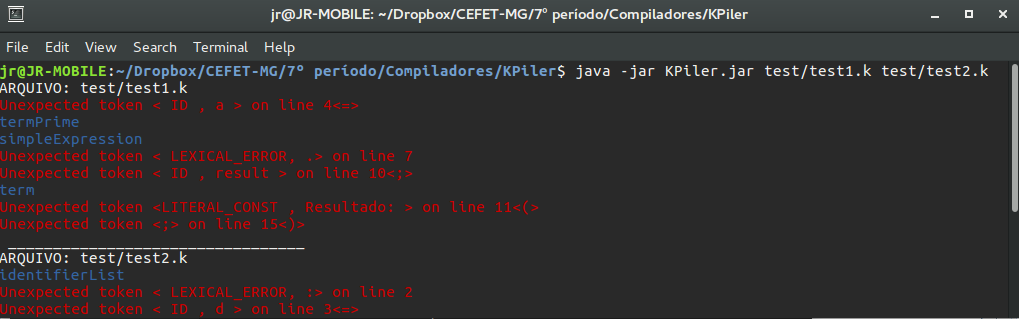
\includegraphics[width=16cm,height=20cm,keepaspectratio]{img/execution.png}
\caption{Execução do programa via terminal.}
\end{figure}

\chapter[Avaliação dos resultados]{Avaliação dos resultados}
\label{cap:avaliacao}

O programa foi submetido a seis testes de compilação. Cinco dos testes foram elaborados pela orientadora deste trabalho e um teste foi elaborado pelo autor. Os arquivos de teste estão disponibilizados em anexo no diretório \textit{test} disponível neste projeto e em sua página do GitHub\footnote{\url{https://github.com/josuerocha/KPiler}}. A página do GitHub se encontra e modo privado até a conclusão da disciplina.

Os testes foram submetidos ao compilador de maneira incremental, isto é, os erros reportados em na fase inicial foram corrigidos e o código submetido novamente de maneira repetida até que não houvessem mais erros.


\section{\textbf{Teste 1}}

\textbf{Código-fonte:}
        
\begin{lstlisting}
program
	int a, b;
	int result;
	float a,x,total;

	a = 2;
	x = .1;
	scan (b);
	scan (y)
	result = (a*b ++ 1) / 2;
	print "Resultado: ";
	print (result);
	print ("Total: ");
	total = y / x;
	print ("Total: ";
	print (total);
end
\end{lstlisting}
        
\textbf{Resultado da execução 1:}
        
 \begin{lstlisting}
Syntax error: unexpected token < ID , a > on line 4
Lexical error: Invalid token . on line 7
Syntax error: unexpected token < ID , result > on line 10
Syntax error: unexpected token <LITERAL_CONST , Resultado: > on line 11
Syntax error: unexpected token <;> on line 15
\end{lstlisting}

Os erros apresentados foram corrigidos com as seguintes modificações:
\begin{itemize}
    \item Substituição da palavra chave \textit{float} por \textit{int} na linha 4;
    
    \item Remoção do . na linha 7;
    
    \item Adição do ; ao final da linha 9;
    
    \item Envolvimento do literal "Resultado" com () na linha 11;
    
    \item Adição de ) após o literal "Total: " na linha 15.
\end{itemize}

O código-fonte submetido ao compilador novamente:

\textbf{Código-fonte corrigido:}
\begin{lstlisting}
program
	int a, b;
	int result;
	int a,x,total;

	a = 2;
	x = 1;
	scan (b);
	scan (y);
	result = (a*b ++ 1) / 2;
	print ("Resultado: ");
	print (result);
	print ("Total: ");
	total = y / x;
	print ("Total: ");
	print (total);
end
\end{lstlisting}

\textbf{Resultado da execução 2:}
\begin{lstlisting}
Syntax error: unexpected token <+> on line 10
\end{lstlisting}

O símbolo + adicional foi removido e o código submetido novamente.
\newpage
\begin{lstlisting}
program
	int a, b;
	int result;
	int a,x,total;

	a = 2;
	x = 1;
	scan (b);
	scan (y);
	result = (a*b + 1) / 2;
	print ("Resultado: ");
	print (result);
	print ("Total: ");
	total = y / x;
	print ("Total: ");
	print (total);
end
\end{lstlisting}

Nenhum outro erro foi retornado pelo compilador após esta alteração, atendendo aos resultados esperados.
    
\section{\textbf{Teste 2}}
    
\textbf{Código-fonte:}

\begin{lstlisting}
program
	int: a, c;
	float d, _e;
	a = 0; d = 3.5
	c = d / 1.2;
	Scan (a);
	Scan (c);
	b = a * a;
	c = b + a * (1 + a*c);
	print ("Resultado: ");
	print c;
	a = b + c + d)/2;
	e = val + c + a;
	print ("E: ");
	print (e);
\end{lstlisting}

\textbf{Resultado de execução:}
        
        
 \begin{lstlisting}
Lexical error: Invalid token : on line 2
Syntax error: unexpected token < ID , d > on line 3
Lexical error: Invalid token . on line 4
Syntax error: unexpected token <(> on line 6
Syntax error: unexpected token <(> on line 7
Syntax error: unexpected token < ID , c > on line 11
Syntax error: unexpected token <)> on line 12
\end{lstlisting}

O programa fonte foi corrigido da seguinte maneira:

\begin{itemize}
    \item O caractere : foi removido da linha 2;
    
    \item A palavra \textit{float} foi substituída por \textit{int} na linha 3;
    
    \item O caractere . foi removido da linha 4;
    
    \item A palavra Scan foi substituida por scan nas linhas 6 e 7;
    
    \item O identificador c na linha 11 foi cercado de ();
    
    \item Foi acrescentado o ( na linha 12.
    
\end{itemize}

\textbf{Código-fonte corrigido:}

\begin{lstlisting}
program
	int a, c;
	int d, _e;
	a = 0; d = 35
	c = d / 1.2;
	scan (a);
	scan (c);
	b = a * a;
	c = b + a * (1 + a*c);
	print ("Resultado: ");
	print (c);
	a = (b + c + d)/2;
	e = val + c + a;
	print ("E: ");
	print (e);
\end{lstlisting}

O código-fonte foi submetido novamente ao compilador:

\begin{lstlisting}
Lexical error: Invalid token _ on line 3
Syntax error: unexpected token < ID , e > on line 3
Syntax error: unexpected token < ID , c > on line 5
Syntax error: unexpected end of file
\end{lstlisting}

Correções:

\begin{itemize}
    \item Remoção do caractere \textunderscore  na linha 3;
    
    \item Adição de ; ao final da linha 4;
    
    \item Adição da palavra reservada end ao final do programa.
\end{itemize}

\textbf{Código-fonte corrigido:}

\begin{lstlisting}
program
	int a, c;
	int d, e;
	a = 0; d = 35;
	c = d / 1.2;
	scan (a);
	scan (c);
	b = a * a;
	c = b + a * (1 + a*c);
	print ("Resultado: ");
	print (c);
	a = (b + c + d)/2;
	e = val + c + a;
	print ("E: ");
	print (e);
end
\end{lstlisting}

Após submissão, o compilador retornou um erro:

\begin{lstlisting}
Lexical error: Invalid token . on line 5
\end{lstlisting}

O caractere . na linha 5 foi removido e submetido novamente:

\textbf{Código-fonte corrigido:}

\begin{lstlisting}
program
	int a, c;
	int d, e;
	a = 0; d = 35;
	c = d / 12;
	scan (a);
	scan (c);
	b = a * a;
	c = b + a * (1 + a*c);
	print ("Resultado: ");
	print (c);
	a = (b + c + d)/2;
	e = val + c + a;
	print ("E: ");
	print (e);
end
\end{lstlisting}

Nenhum erro foi retornado, atendendo aos resultados esperados.

\section{\textbf{Teste 3}}
    
        \textbf{Código-fonte:}
        
        \begin{lstlisting}
    program
    	int pontuacao, pontuacaoMaxima, disponibilidade;
    	string pontuacaoMinima;
    	disponibilidade = "Sim";
    	pontuacaoMinima = 50;
    	pontuacaoMaxima = 100;
    	/* Entrada de dados
    	Verifica aprovação de candidatos
    	do
    	print("Pontuacao Candidato: ");
    		scan(pontuacao);
    		print("Disponibilidade Candidato: ");
    		scan(disponibilidade);
    
    		if ((pontuação > pontuacaoMinima) and (disponibilidade=="Sim") then
    			print("Candidato aprovado");
    		else
    			print("Candidato reprovado")
    		end
    	while (pontuação >= 0)end
    end
        \end{lstlisting}
        
        \textbf{Resultado de execução:}
        
        
 \begin{lstlisting}
Lexical error: Unclosed multiple line comment on line 7
\end{lstlisting}

O compilador retornou erro de comentário não fechado na linha sete do programa fonte. Para corrigir, o comentário foi fechado na linha 8.

        \textbf{Código-fonte:}
        
        \begin{lstlisting}
 program
	int pontuacao, pontuacaoMaxima, disponibilidade;
	string pontuacaoMinima;
	disponibilidade = "Sim";
	pontuacaoMinima = 50;
	pontuacaoMaxima = 100;
	/* Entrada de dados
	Verifica aprovação de candidatos */
	do
	print("Pontuacao Candidato: ");
	scan(pontuacao);
	print("Disponibilidade Candidato: ");
	scan(disponibilidade);

	if ((pontuação > pontuacaoMinima) and (disponibilidade=="Sim") then
		print("Candidato aprovado");
	else
		print("Candidato reprovado")
	end
	while (pontuação >= 0) end
end
        \end{lstlisting}
        
O código-fonte foi submetido novamente:
\textbf{Resultado de execução:}

\begin{lstlisting}
Syntax error: unexpected token < ID , and > on line 15
Syntax error: unexpected token < END > on line 19
\end{lstlisting}

Medidas corretivas:

\begin{itemize}
	\item Substituição da palavra and pelo operador \&\& na linha 15;
	
	\item Adição de ; ao final da linha 18.

\end{itemize}

\newpage

\textbf{}
\begin{lstlisting}
program
	int pontuacao, pontuacaoMaxima, disponibilidade;
	string pontuacaoMinima;
	disponibilidade = "Sim";
	pontuacaoMinima = 50;
	pontuacaoMaxima = 100;
	/* Entrada de dados
	Verifica aprovação de candidatos */
	do
	print("Pontuacao Candidato: ");
		scan(pontuacao);
		print("Disponibilidade Candidato: ");
		scan(disponibilidade);

		if ((pontuação > pontuacaoMinima) && (disponibilidade=="Sim") then
			print("Candidato aprovado");
		else
			print("Candidato reprovado");
		end
	while (pontuação >= 0) end
end
\end{lstlisting}

\textbf{Resultado de execução:}

\begin{lstlisting}
Syntax error: unexpected token < THEN > on line 15
\end{lstlisting}

Um ) foi adicionado à linha 15 para fechar a expressão como medida corretiva.

\textbf{Código-fonte corrigido}

\begin{lstlisting}
program
	int pontuacao, pontuacaoMaxima, disponibilidade;
	string pontuacaoMinima;
	disponibilidade = "Sim";
	pontuacaoMinima = 50;
	pontuacaoMaxima = 100;
	/* Entrada de dados
	Verifica aprovação de candidatos */
	do
	print("Pontuacao Candidato: ");
		scan(pontuacao);
		print("Disponibilidade Candidato: ");
		scan(disponibilidade);

		if ((pontuação > pontuacaoMinima) && (disponibilidade=="Sim")) then
			print("Candidato aprovado");
		else
			print("Candidato reprovado");
		end
	while (pontuação >= 0) end
end
\end{lstlisting}

O resultado esperado foi alcançado, pois o compilador reportou conclusão com sucesso.

\newpage


\section{\textbf{Teste 4}}
    
    O código fonte inicial foi submetido ao compilador:
        \textbf{Código-fonte:}
        
        \begin{lstlisting}
    		int: a, aux$, b;
        	string nome, sobrenome, msg;
        	print(Nome: );
        	scan (nome);
        	print("Sobrenome: ");
        	scan (sobrenome);
        	msg = "Ola, " + nome + " " +
        	sobrenome + "!";
        	msg = msg + 1;
        	print (msg);
        	scan (a);
        	scan(b);
        	if (a>b) then
        		aux = b;
        		b = a;
        		a = aux;
        	end;
        	print ("Apos a troca: ");
        	out(a);
        	out(b)
        end
        \end{lstlisting}
        
        \textbf{Resultado de execução:}
        
 \begin{lstlisting}
Syntax error: unexpected token < INT > on line 1
\end{lstlisting}

O programa fonte apresentou erro na linha 1, pois a palavra chave program não foi introduzida ao início do programa. O programa foi corrigido e submetido novamente.

\textbf{Código-fonte corrigido:}

\begin{lstlisting}
program
	int: a, aux$, b;
	string nome, sobrenome, msg;
	print(Nome: );
	scan (nome);
	print("Sobrenome: ");
	scan (sobrenome);
	msg = "Ola, " + nome + " " +
	sobrenome + "!";
	msg = msg + 1;
	print (msg);
	scan (a);
	scan(b);
	if (a>b) then
		aux = b;
		b = a;
		a = aux;
	end;
	print ("Apos a troca: ");
	out(a);
	out(b)
end
\end{lstlisting}

\textbf{Resultado de execução:}

 \begin{lstlisting}
Lexical error: Invalid token : on line 2
Lexical error: Invalid token : on line 4
Syntax error: unexpected token <;> on line 18
\end{lstlisting}

O código-fonte foi corrigido de acordo com os seguintes procedimentos:

\begin{itemize}
    \item O caractere : foi removido na linha 2;
    
    \item O caractere : foi removido na linha 4.
    
    \item o caractere ; foi removido da linha 18
\end{itemize}

\textbf{Código-fonte corrigido:}
\begin{lstlisting}
program	
	int a, aux$, b;
	string nome, sobrenome, msg;
	print(Nome );
	scan (nome);
	print("Sobrenome: ");
	scan (sobrenome);
	msg = "Ola, " + nome + " " +
	sobrenome + "!";
	msg = msg + 1;
	print (msg);
	scan (a);
	scan(b);
	if (a>b) then
		aux = b;
		b = a;
		a = aux;
	end
	print ("Apos a troca: ");
	out(a);
	out(b)
end
\end{lstlisting}

\textbf{Resultado da execução:}
\begin{lstlisting}
Lexical error: Invalid token $ on line 2
Syntax error: unexpected token < ID , b > on line 2
Syntax error: unexpected token < STRING > on line 3
\end{lstlisting}

O token inválido \$ foi a causa de todos os três erros. O token \$ foi removido e o programa submetido novamente:

\textbf{Código-fonte corrigido:}
\begin{lstlisting}
program	
	int a, aux, b;
	string nome, sobrenome, msg;
	print(Nome );
	scan (nome);
	print("Sobrenome: ");
	scan (sobrenome);
	msg = "Ola, " + nome + " " +
	sobrenome + "!";
	msg = msg + 1;
	print (msg);
	scan (a);
	scan(b);
	if (a>b) then
		aux = b;
		b = a;
		a = aux;
	end
	print ("Apos a troca: ");
	out(a);
	out(b)
end
\end{lstlisting}

\textbf{Resultado da execução:}
\begin{lstlisting}
Syntax error: unexpected token <(> on line 20
Syntax error: unexpected token <(> on line 21
\end{lstlisting}

Foram detectados erros nas linhas 20 e 21 devido à utilização de um comando (out) inválido que foi detectado como identificador. A palavra \textit{out} foi substituída pela palavra chave \textit{print}:

\textbf{Código-fonte corrigido:}
\begin{lstlisting}
program	
	int a, aux, b;
	string nome, sobrenome, msg;
	print(Nome );
	scan (nome);
	print("Sobrenome: ");
	scan (sobrenome);
	msg = "Ola, " + nome + " " +
	sobrenome + "!";
	msg = msg + 1;
	print (msg);
	scan (a);
	scan(b);
	if (a>b) then
		aux = b;
		b = a;
		a = aux;
	end
	print ("Apos a troca: ");
	print(a);
	print(b)
end
\end{lstlisting}

O programa-fonte foi testado novamente:

\begin{lstlisting}
Syntax error: unexpected token < END > on line 22
\end{lstlisting}

Este erro foi corrigido adicionando-se o ; ao final da linha 21.

\begin{lstlisting}
program	
	int a, aux, b;
	string nome, sobrenome, msg;
	print(Nome );
	scan (nome);
	print("Sobrenome: ");
	scan (sobrenome);
	msg = "Ola, " + nome + " " +
	sobrenome + "!";
	msg = msg + 1;
	print (msg);
	scan (a);
	scan(b);
	if (a>b) then
		aux = b;
		b = a;
		a = aux;
	end
	print ("Apos a troca: ");
	print(a);
	print(b);
end
\end{lstlisting}

A execução atendeu aos resultados esperados não retornando outros erros.

\section{\textbf{Teste 5}}
    
\textbf{Código-fonte:}

\begin{lstlisting}
program
	int a, b, c, maior, outro;

	do
		print("A");
		scan(a);
		print("B");
		scan(b);
		print("C");
		scan(c);
		//Realizacao do teste
		if ( (a>b) && (a>c)
			maior = a
		)
		else
		if (b>c) then
			maior = b;
		else
			maior = c;
		end
		end
		print("Maior valor:"");
		print (maior);
		print ("Outro? ");
		scan(outro);
	while (outro >= 0)
end
\end{lstlisting}

\textbf{Resultado de execução:}
        
\begin{lstlisting}
Syntax error: unexpected token < ID , maior > on line 13
Syntax error: unexpected token < ELSE > on line 15
Syntax error: unexpected token <)> on line 16
Syntax error: unexpected token < END > on line 21
\end{lstlisting}

O programa fonte foi corrigido de acordo com as seguintes alterações:

\begin{itemize}
    \item Adição de ) e a palavra reservada \textit{then} ao fim da linha 12;
    
    \item Remoção do ) na linha 14 (correção do segundo erro).
    
\end{itemize}

\textbf{Correção}
 \begin{lstlisting}
program
	int a, b, c, maior, outro;

	do
		print("A");
		scan(a);
		print("B");
		scan(b);
		print("C");
		scan(c);
		//Realizacao do teste
		if ( (a>b) && (a>c)) then
			maior = a
		else
		if (b>c) then
			maior = b;
		else
			maior = c;
		end
		end
		print("Maior valor:"");
		print (maior);
		print ("Outro? ");
		scan(outro);
	while (outro >= 0)
end

\end{lstlisting}

\textbf{Resultado:}

 \begin{lstlisting}
Syntax error: unexpected token < ELSE > on line 14
Syntax error: unexpected token <>> on line 15
Syntax error: unexpected token < END > on line 20\end{lstlisting}

Para corrigir os erros o ; foi adicionado ao final da linha 13.

\begin{lstlisting}
program
	int a, b, c, maior, outro;

	do
		print("A");
		scan(a);
		print("B");
		scan(b);
		print("C");
		scan(c);
		//Realizacao do teste
		if ( (a>b) && (a>c)) then
			maior = a;
		else
		if (b>c) then
			maior = b;
		else
			maior = c;
		end
		end
		print("Maior valor:"");
		print (maior);
		print ("Outro? ");
		scan(outro);
	while (outro >= 0)
end

\end{lstlisting}

\textbf{Resultado de execução:}
\begin{lstlisting}
Lexical error: Unclosed string literal on line 21
Syntax error: unexpected end of file.
\end{lstlisting}

Para fazer as correções o símbolo \detokenize{"}  foi removido da linha 21 para evitar abertura errônea de \textit{string} literal e o símbolo end foi adicionado à linha 25 para corrigir o erro de fim de arquivo inesperado.

\textbf{Código-fonte corrigido:}
\begin{lstlisting}
program
	int a, b, c, maior, outro;

	do
		print("A");
		scan(a);
		print("B");
		scan(b);
		print("C");
		scan(c);
		//Realizacao do teste
		if ( (a>b) && (a>c)) then
			maior = a;
		else
		if (b>c) then
			maior = b;
		else
			maior = c;
		end
		end
		print("Maior valor:");
		print (maior);
		print ("Outro? ");
		scan(outro);
	while (outro >= 0) end
end
\end{lstlisting}


Os erros apresentados anteriormente foram resolvidos, atendendo aos resultados esperados.

\section{\textbf{Teste 6}}
    
        \textbf{Código-fonte:}
        
        \begin{lstlisting}
    	/*THIS IS A MULTIPLE LINE COMMENT
        Josué Rocha Lima */
        
        program
        	//this is an unclosed string literal
        	string str = "HELLO WORLD"
        	int 20 = 20;
        
        	for i = 0 : str.size()
        		print(i);
        	end
        
        end
        \end{lstlisting}
        
        \textbf{Resultado de execução:}
        
 \begin{lstlisting}
Syntax error: unexpected token <=> on line 6
Syntax error: unexpected token < ID , for > on line 9
Syntax error: unexpected token <)> on line 9
\end{lstlisting}

Correção dos erros:

\begin{itemize}
    \item Separação da declaração e atribuição de valor às variáveis;
    
    \item Troca do for por do e outras adaptações necessárias;
    
    \item Substituição de str.size() por um identificador.
\end{itemize}

\begin{lstlisting}
/*THIS IS A MULTIPLE LINE COMMENT
Josué Rocha Lima */

program
	//this is an unclosed string literal
	string str;
	int i;
	int maxtam;
	
	maxtam = 20;
	str = "HELLO WORLD";
	
	do 
		print(i);
		i = i + 1;
	while i < maxtam end

end
\end{lstlisting}

O programa fonte não apresentou erros, correspondendo aos resultados esperados.








\chapter[Conclusão]{Conclusão}
\label{cap:conclusao}

O trabalho em questão contribuiu para o entendimento dos fundamentos e técnicas de análise sintática por meio do desenvolvimento do software compilador \textit{KPiler}. Percebeu-se a importância do analisador sintático para o compilador como núcleo do mesmo.

Experiências durante esta implementação facilitaram o entendimento do funcionamento dos analisadores sintáticos presentes em compiladores comerciais, bem como suas mensagens de erro.

Todos os resultados de testes aplicados ao \textit{KPiler} atenderam aos resultados esperados, quanto à coerência da informação reportada e quanto ao tempo de execução.


% ----------------------------------------------------------








% ----------------------------------------------------------
% Finaliza a parte no bookmark do PDF
% para que se inicie o bookmark na raiz
% e adiciona espaço de parte no Sumário
% ----------------------------------------------------------
% \phantompart







% ----------------------------------------------------------
% ELEMENTOS PÓS-TEXTUAIS
% ----------------------------------------------------------

%% Baseado no arquivo: 
%% abtex2-modelo-trabalho-academico.tex, v-1.9.6 laurocesar
%% by abnTeX2 group at http://www.abntex.net.br/ 
%% Adaptado para um modelo de TCC (Graduação)

\postextual

% ----------------------------------------------------------

% ----------------------------------------------------------
% Referências bibliográficas
% ----------------------------------------------------------
\bibliography{relatorio_Lexico_JosueRL}





\end{document}
